%&../settings/preamble.main

\ifsubfile
\usepackage[newfloat, cachedir=_minted-cache, outputdir=../build]{minted}
\usepackage{../libraries/set-minted}
\mintedpath{{../assets/codes/04/}}

\pagestyle{plain}
\setcounter{chapter}{14}

% arara: pdflatex: { options: ["--output-directory=../build"], shell: yes, draft: yes, synctex: no }
% arara: pdflatex: { options: ["--output-directory=../build"], shell: yes, synctex: no }
\begin{document}
\fi
\chapter{Ricerca locale}

E' una tecnica di programmazione. L'idea generale è la seguente: se si conosce una soluzione ammissibile (non necessariamente ottima) ad un problema di ottimizzazione, si può cercare di trovare una soluzione migliore nelle \enquote{vicinanze} di quella precedente.
Si continua in questo modo fino a quando non si è più in grado di migliorare

\begin{minipage}{.6\linewidth}
	\begin{algorithm*}[H]
	\caption{Logica della ricerca locale}
	\SetKwFunction{ricercaLocale}{ricercaLocale}

	\prototype{\ricercaLocale}{
		\(Sol =\) una soluzione ammissibile del problema\;

		\BlankLine
		\While{\(\exists S \in I(Sol)\) migliore di \(Sol\)}{
			\(Sol = S\)
		}
	}

\end{algorithm*}
\end{minipage}
\begin{minipage}{.4\linewidth}
\centering
	\pgfplotsset{width=5cm}
	\begin{tikzpicture}
	\begin{axis}[
		,axis lines = none
		% ,xlabel = \(x\)
		% ,ylabel = {\(f(x)\)}
		% ,legend style={legend pos=south west}
	]
	\addplot [
		smooth,
		% samples=100,
		% mark min,
		domain=-1:4,
		color=darker,
	]
	{3*x^4 - 16*x^3 + 18*x^2};
	% \addlegendentry{\(3x^4 - 16x^3 + 18x^2\)}
	\end{axis}
	\end{tikzpicture}
\end{minipage}

\section{Problema di flusso massimo}

Prima di definire il problema abbiamo bisogno di definire alcune entità e le corrispondenti proprietà.

\begin{minipage}[b]{.5\linewidth}
	\begin{definition}[rete di flusso]
	Una rete di flusso \(G = (V,E,s,t,c)\) è data da:
	\begin{itemize}
		\item un grafo orientato \(G = (V,E)\);
		\item un nodo \(s \in V\) detto \alert{sorgente};
		\item un nodo \(t \in V\) detto \alert{pozzo};
		\item una funzione di \alert{capacità} \(c \colon V \times V \to \mathbb{R}^{\geqslant 0}\),\\tale per cui \((u,v) \not\in R \Rightarrow c(u,v) = 0\).
	\end{itemize}
	\end{definition}
\end{minipage}
\begin{minipage}[b]{.5\linewidth}
% \centering
% \begin{figure}[H]
	% \centering
	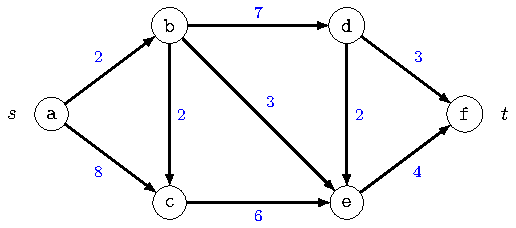
\includegraphics{template}
	% \caption{Rete di flusso}%
	% \label{gif:rete-flusso}
% \end{figure}
\end{minipage}

\begin{definition}
Un flusso in \(G\) è una funzione \(f\colon V \times V \to \mathbb{R}\) (nota che può essere anche negativo) che gode delle seguenti proprietà:
\begin{semicompactlist}
	\item Vincolo sulla capacità;
	\item Antisimmetria;
	\item Conservazione del flusso.
\end{semicompactlist}
\end{definition}

% \bigskip
\begin{minipage}{.5\linewidth}
	\subparagraph{Vincolo sulla capacità}
	Il flusso non deve eccedere la capacità sull'arco, ovvero
	\begin{equation*}
	\forall u,v \in V: f(u,v) \leqslant c(u,v)
	\end{equation*}
\end{minipage}
\begin{minipage}{.5\linewidth}
\centering
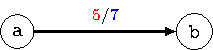
\includegraphics{prop1}
\end{minipage}

\bigskip
\begin{minipage}{.5\linewidth}
	\subparagraph{Antisimmetria}
	Il flusso che passa dal nodo \(u\) al nodo \(v\), è pari a meno il flusso dal nodo \(v\) al nodo \(u\), ovvero
	\begin{equation*}
	\forall u,v \in V: f(u,v) = -f(v,u)
	\end{equation*}
	% NOTE tolto per problemi di spaziatura
	% Il flusso viene definito in questo modo per semplificare la proprietà successiva e altre regole.
\end{minipage}
\begin{minipage}{.5\linewidth}
\centering
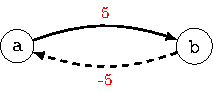
\includegraphics{prop2}
\end{minipage}

\bigskip
\begin{minipage}{.5\linewidth}
	\subparagraph{Conservazione del flusso}

	Per ogni nodo, la somma dei flussi entranti deve essere uguale alla somma dei flussi uscenti.
	\begin{equation*}
	\forall u \in V - \{s, t\} \colon \sum_{v \in V} f(u, v) = 0
	\end{equation*}
	La sommatoria dei flussi che partono da \(u\) a qualunque altro nodo, ad esclusione della sorgente e del pozzo, deve essere 0.
\end{minipage}
\begin{minipage}{.5\linewidth}
\centering
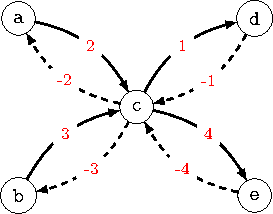
\includegraphics{prop3}
\end{minipage}

\begin{definition}[valore del flusso]
Il valore di un flusso \(f\) è definito come la quantità di flusso uscente da \(s\).
\begin{equation*}
\abs{f} = \sum_{\mathclap{(s,v) \in E}}\; f (s,v)
\end{equation*}
\end{definition}

\subsection{Problema del flusso massimo}

\begin{definition}[Flusso massimo]
Data una rete \(G = (V, E, s, t, c)\), trovare un flusso che abbia valore massimo fra tutti i flussi associabili alla rete.
\begin{equation*}
\abs{f^{*}} = \max\{\, \abs{f}\, \}
\end{equation*}
\end{definition}

\begin{comment}
\begin{minipage}[t]{.45\linewidth}\centering
	\begin{figure}[H]
		\centering
		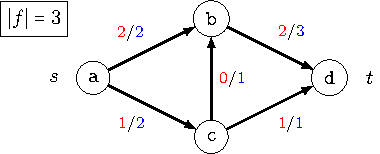
\includegraphics{esempioFlusso}
		\caption{Il valore del flusso in questo caso è pari a \(3\) ma non è massimo}%
		\label{gif:valore-flusso}
	\end{figure}
\end{minipage}\hfill
\begin{minipage}[t]{.45\linewidth}\centering
	\begin{figure}[H]
		\centering
		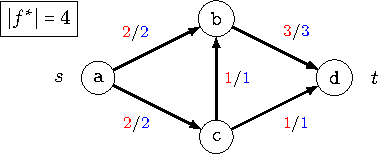
\includegraphics{esempioFlusso-maxFlow}
		\caption{Il valore del flusso massimo per questa rete è \(4\)}
		\label{gif:flusso-massimo}
	\end{figure}
\end{minipage}
\end{comment}

\begin{figure}[H]
	\begin{subfigure}[t]{0.475\textwidth}\centering
		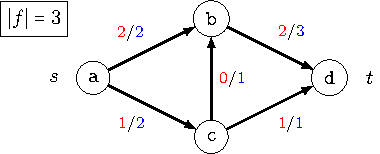
\includegraphics{esempioFlusso}
		\caption{Il valore del flusso in questo caso è pari a \(3\) ma non è massimo.}
		\label{gif:valore-flusso}
	\end{subfigure}\hfill
	\begin{subfigure}[t]{0.475\textwidth}\centering
		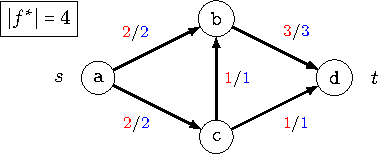
\includegraphics{esempioFlusso-maxFlow}
		\caption{Il valore del flusso massimo per questa rete è \(4\).}
		\label{gif:flusso-massimo}
	\end{subfigure}
	% \caption{Principali topologie dei modelli compartimentali.}
	% \label{fig:main}
\end{figure}

\begin{note}
Il nostro obiettivo è quindi quello di trovare il flusso massimo.
\end{note}

\section{Metodo delle reti residue}

Utilizziamo quindi il \emph{metodo delle reti residue}.
Il metodo consiste nel partire da un flusso \enquote{corrente} \(f\), inizialmente nullo e
\begin{enumerate*}[label=\arabic*)]
	\item si \enquote{sottrae} il flusso attuale dalla rete iniziale, ottenendo così una rete residua;
	\item si cerca un flusso \(g\) all'interno della rete residua;
	\item si somma \(g\) ad \(f\).
\end{enumerate*}, ripetendo le azioni precedenti fino a quando non è più possibile trovare un flusso positivo \(g\).

Se il procedimento viene svolto correttamente, è possibile dimostrare che questo approccio restituisce un flusso massimo.

\begin{note}
\`{E} un algoritmo di ricerca locale, senza una dimostrazione non è possibile dire che la soluzione sia ottima.
\end{note}

\begin{definition}[Flusso nullo]
Definiamo \alert{flusso nullo} la funzione \(f_0 \colon V \times V \to R^{\leqslant 0}\) tale che \(f(u,v) = 0\) per ogni \(u, v \in V\).
\end{definition}

\begin{definition}[Somma di flussi]
Per ogni coppia di flussi \(f_1\) e \(f_2\) in \(G\), definiamo il \alert{flusso somma} \(g = f_1 + f_2\) come un flusso tale per cui \(g(u,v) = f_1(u,v) + f_2(u,v)\)
\end{definition}
\begin{note}
\`{E} possibile invalidare il vincolo sulla capacità.
\end{note}

\begin{minipage}{.5\linewidth}
\begin{definition}[Capacità residua]
	Definiamo \alert{capacità residua} di un flusso \(f\) una funzione \mbox{\(c_{f}\colon V \times V \to R^{\geqslant 0}\)} tale che \(c_{f}(u,v) = c(u,v) - f(u,v)\)
	\end{definition}
	Per la definizione di capacità residua, si creano degli archi all'indietro: \(c_{f}(b,a) = c(b,a) - f(b,a) = 0 - (-5) = 5\)
\end{minipage}
\begin{minipage}{.5\linewidth}\centering
	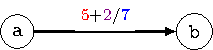
\includegraphics{prop4}
\end{minipage}

\begin{minipage}{.5\linewidth}
	\begin{definition}[Reti residue]
	Data una rete di flusso \(G = (V, E, s, t, c)\) e un flusso \(f\) su \(G\), possiamo costruire una \alert{rete residua} \(G_f = (V, \alert{E_f}, s, t, \alert{c_f})\), tale per cui \((u,v) \in E_f\) se e solo se \(c_f(u,v) > 0\).
	\end{definition}
\end{minipage}
\begin{minipage}{.5\linewidth}
	\centering
	% \begin{figure}[H]
	% \centering
	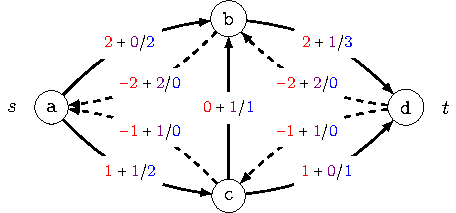
\includegraphics{reteResidua}
	% \caption{Rete residua}%
	% \label{gif:valore-flusso}
	% \end{figure}
\end{minipage}

\subsection{Algoritmo}

\begin{algorithm}[H]
\caption{Schema generale}

\SetKwFunction{maxFlow}{maxFlow}

\prototype{\Matrix{\Int} \maxFlow{\Graph G, \Node s, \Node t, \Matrix{\Int} c}}{

	\BlankLine
	\(f \Assign f_0\) \Comment*[h]{inizializza un flusso nullo}
	\(r \Assign c\) \Comment*[h]{capacità iniziale}

	\BlankLine
	\tcp{Fintanto che non rimane un flusso nullo}
	\Repeat{\(g \Equal f_0\)}{
		\(g \Assign\) trova un flusso \(r\) tale che \(\abs{g} > 0\), altrimenti \(f_0\)\;
		\AddTo{f}{g} \Comment*[h]{necessita di una dimostrazione}\;
		\(r \Assign\) rete di flusso residua del flusso \(f\) in \(G\)\;

	}

	\BlankLine
	\Return \(f\) \Comment*[h]{il flusso}\;
}

\end{algorithm}

\paragraph{Dimostrazione di correttezza}
\begin{lemma}
Se \(f\) è un flusso in \(G\) e \(g\) è un flusso in \(G_f\), allora \(f + g\) è un flusso in \(G\).
\end{lemma}

\subparagraph{Vincolo sulla capacità}

\begin{proof}
\[\begin{WithArrows}
g(u,v) &\leqslant c_f(u,v) \Arrow{sostituisco \(c_f\)} \\
%
g(u,v) &\leqslant c(u,v) - f(u,v) \Arrow{aggiungo termine uguale} \\
%
\mathcolor{mathcolor}{f(u,v)} + g(u,v) &\leqslant c(u,v) - \Ccancel{f(u,v)} + \Ccancel{\mathcolor{mathcolor}{f(u,v)}} \Arrow{raccolgo e semplifico} \\
%
(\mathcolor{mathcolor}{f} + g)(u,v) &\leqslant c_f(u,v)
\end{WithArrows}\]
\end{proof}

% TODO vincolo sulla capacità
\subparagraph{Vincolo sulla capacità}

\texttt{MATERIALE MANCANTE}

% TODO indicare il numero delle slide
\subparagraph{Esempio}
Fare riferimento alla spiegazione grafica (\href{https://youtu.be/rxH0SEakE2Y?t=2127}{minuto 35:27}) qui non riportata (riferimento trasparenze \slide{00} - \slide{00}.

% TODO scrivere algoritmo
\begin{algorithm}[H]
	\caption{Algoritmo di Ford-Fulkerson}
	%&../preamble

% \documentclass[varwidth=6in]{standalone}
% \usepackage{../preamble}

% arara: pdflatex: { synctex: no }
% arara: latexmk: { clean: partial }
\ifstandalone
\begin{document}
\NoCaptionOfAlgo
\begin{algorithm}[H]
\caption[]{}
\fi

\SetKwFunction{nomeFunzione}{nomeFunzione}

\prototype{\Int \nomeFunzione{parameters}}{
	\BlankLine


	\BlankLine
	\Return \(0\)\;
}

\ifstandalone
\end{algorithm}
\RestoreCaptionOfAlgo
\end{document}
\fi

\end{algorithm}

\subparagraph{Ricerca del cammino}
Manca del testo.
Notare che le due cose non si escludono a vicenda.
Il costo della visita è \(\Omicron(V+E)\).

\begin{code}
\captionof{listing}{inserire didascalia}
\begin{minted}{java}
/**
 * Compute the max-flow using the Ford-Fulkerson algorithm
 * @param C the capacity matrix
 * @param s the source node
 * @param t the sink node
 * @return the flow matrix
 */
private static int[][] flow(int[][] C, int s, int t) {
	// Create an empty flow
	int[][] F = new int[C.length][C.length];

	// Visited array to perform DFS, initially empty
	boolean[] visited = new boolean[C.length];

	// Repeat until there is no path
	while (dfs(C, F, s, t, visited, Integer.MAX_VALUE) > 0) {
		Arrays.fill(visited, false);
	}
	return F;
}
\end{minted}
\end{code}

\begin{code}
\captionof{listing}{inserire didascalia}
\begin{minted}{java}
/**
 * Performs a DFS starting from node i and trying to reach node t.
 * @param C the capacity matrix; if capacity[x][y]>0, there is a edge from x to y
 * @param F the flow matrix to be computed
 * @param i the current node,
 * @param t the sink node
 * @param visited the boolean set containing the nodes that have been visited
 * @param min the smallest capacity found during the visit.
 * @returns the value of the additional flow found during the DFS
 */
private static int dfs(int[][] C, int[][] F, int i, int t, boolean[] visited, int min) {
	// If sink has been reached, terminate
	if (i == t) return min;

	visited[i] = true;
	for (int j = 0; j < C.length; j++) {
		if (C[i][j] > 0 && !visited[j]) {
			// Non-visited neighbor
			int val = dfs(C, F, j, t, visited, Math.min(min, C[i][j]));
			if (val > 0) {
				C[i][j] = C[i][j] - val;
				C[j][i] = C[j][i] + val;

				F[i][j] = F[i][j] + val;
				F[j][i] = F[j][i] - val;

				return val;
			}
		}
	}

	// The sink has not been found
	return 0;
}
\end{minted}
\end{code}

\paragraph{Complessità}
Se le capacità della rete sono intere, l'algoritmo di Ford e Fulkerson ha complessità \(\Omicron((V+E)\, \abs{f^{*}} )\) (il costo della visita in ampiezza) o complessità \(\Omicron(V^2\, \abs{f^{*}}) \) nel caso pessimo (se fatto su una matrice).

L'algoritmo di Edmonds e Karp ha complessità \(\Omega(V \cdot E^{2})\) nel caso pessimo.

Entrambi i limiti superiori sono validi, si prende quindi il più basso fra i due.

\begin{note}
Il cambio di notazione (ovvero segnalare i nodi con \(V\) (\emph{vertex}) anziché con \(n\), e i lati con \(E\) (\emph{edges}) anziché con \(m\)) è necessario per non fare confusione con gli esercizi.
\end{note}

\begin{lemma}
Il numero totale di aumenti di flusso eseguiti dall'algoritmo di Edmonds e Karp è \(\Omicron(V \cdot E) \).
\end{lemma}

\subsection{Dimostrazione complessità}

\texttt{MATERIALE MANCANTE}
% Omessa.
%
% Tabella delle complessità.
%
% Dinic è il più utilizzato.
% In Ordin i fattori moltiplicativi sono importanti.

\subsection{Dimostrazione correttezza}

Per fare la dimostrazione di correttezza dobbiamo (re)introdurre delle definizioni.

\begin{definition}[Taglio]
Un \alert{taglio} (S,T) della rete di flusso \(G = (V,E,s,t,c)\) è una partizione \(V\) in \(S\) e \(T = V-S\) tale che \(s \in S\), \(t \in T\).
\end{definition}

Mettere schema a destra.

\begin{definition}[Capacità di un taglio]
La \alert{capacità} \(c(S,T)\) attraverso il taglio \(S,T\) è pari a
\begin{equation*}
c(S,T) = \sum_{\mathclap{u \in S, v \in T}}\; c(u,v)
\end{equation*}
\end{definition}

Mettere schema a destra.

\begin{definition}[Flusso di un taglio]
Se \(f\) è un \alert{flusso} in \(G\), il flusso netto \(F(S,T)\) attraverso \((S,T)\) è  pari a
\begin{equation*}
F(S,T)= \sum_{\mathclap{u \in S, v \in T}}\; f(u,v)
\end{equation*}
\end{definition}

Mettere schema a destra.

\begin{lemma}[Valore del flusso di un taglio]
Dato un flusso \(f\) e un taglio \((S,T)\), la quantità di flusso \(F(S,T)\) che attraversa il taglio è uguale a \(\abs{f}\).
\end{lemma}

% TODO trovare l'errore
\[\begin{WithArrows}[displaystyle]
F(S,T) &= \sum_{\mathclap{u \in S, v \in T}}\; f(u,v) \Arrow{\(V = T - S\)} \\
       &= \sum_{\mathclap{u \in S, v \in \mhl{V}}}\; f(u,v) - \sum_{\mathclap{u, v \in \mhl{S}}}\; f(u,v) \Arrow{conservazione del flusso\\ e antisimmetria} \\
	   &= \underbracket[1pt]{\sum_{\mathclap{u \in S \mhl{-\{s\}}, v \in V}}\; f(u,v)}_{0}%
	      + \sum_{\mathclap{v \in V}}\; f(\mhl{s},v)%
		  + \underbracket[1pt]{\sum_{\mathclap{u, v \in S}}\; f(u,v)}_{0} \Arrow{per definizione} \\
	   &= \sum_{\mathrlap{v \in V}}\; f(s,v) = f
\end{WithArrows}\]
% dove \(\displaystyle \sum_{\mathclap{u \in S \mhl{-\{s\}}, v \in V}}\; f(u,v) = 0\) per la conservazione del flusso, e \(\displaystyle \sum_{\mathclap{u \in S , v \in S}}\; f(u,v) = 0\) per antisimmetria.

Un taglio definisce un limite superiorie al flusso massimo che può essere presente nella rete.

\begin{lemma}[Capacità del taglio]
Il flusso massimo è limitato superiormente dalla capacità del taglio minimo (ovvero il taglio la cui capacità è minotr fra tutti i taglio).
\end{lemma}

\texttt{MATERIALE MANCANTE}
% Mettere schema a destra.

La somma dei flussi dev'essere necessariamente minore della somma delle capacità.

\texttt{MATERIALE MANCANTE}
% Riporta equazione.

Quindi, il valore del flisso è limitato superiormente dalla capacità di tutti i possibili tagli.

\begin{theorem}[Teorema del flusso massimo]
Le seguenti affermazioni sono equivalenti:
\begin{itemize}
	\item a
	\item b
	\item c
\end{itemize}
\end{theorem}

\texttt{DA FINIRE}

\ifsubfile
\end{document}
\fi
